\subsection{Energy lab}\label{sc:energylab}

To test the energy consumption of the nodes, a laboratory test has been conducted on two telosB units. On figure \ref{fig:energyLab_testSetup} the test setup is defined. The test was conducted with the same method as laboratory exercise 5\footnote{\cite{Madsen}}. Data and pictures can be found in Appendix7, codes for conducting the laboratory experiments can be found in Appendix8.

\noindent The measurements can be seen on figure \ref{fig:radioOn_idle}, \ref{fig:radioOn_sendHighSignal}, \ref{fig:radioOn_sendMidSignal} and \ref{fig:radioOn_sendLowSignal}. Inspecting the values of the three signal strengths on figure \ref{fig:radioOn_idle}, \ref{fig:radioOn_sendHighSignal}, \ref{fig:radioOn_sendMidSignal} and \ref{fig:radioOn_sendLowSignal}, and converting these voltages to a current, provides the results found in table \ref{tab:signalStrengthEnergyConsumption}.

\begin{figure}[H]
	\centering
	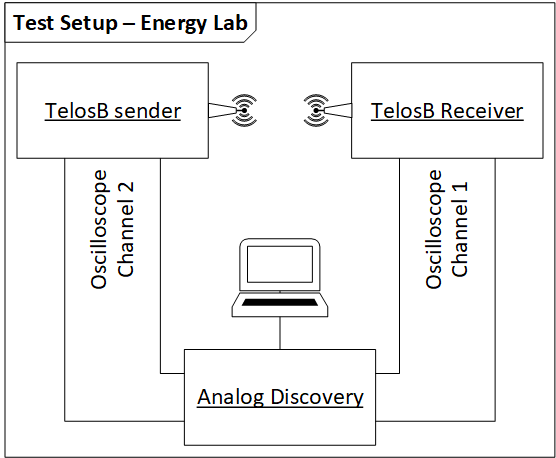
\includegraphics[width=1\linewidth]{implementation/energylab/fig/energyLab_testSetup.png}
	\caption{Energy lab test setup.}
	\label{fig:energyLab_testSetup}
\end{figure}

\begin{figure}[H]
	\centering
	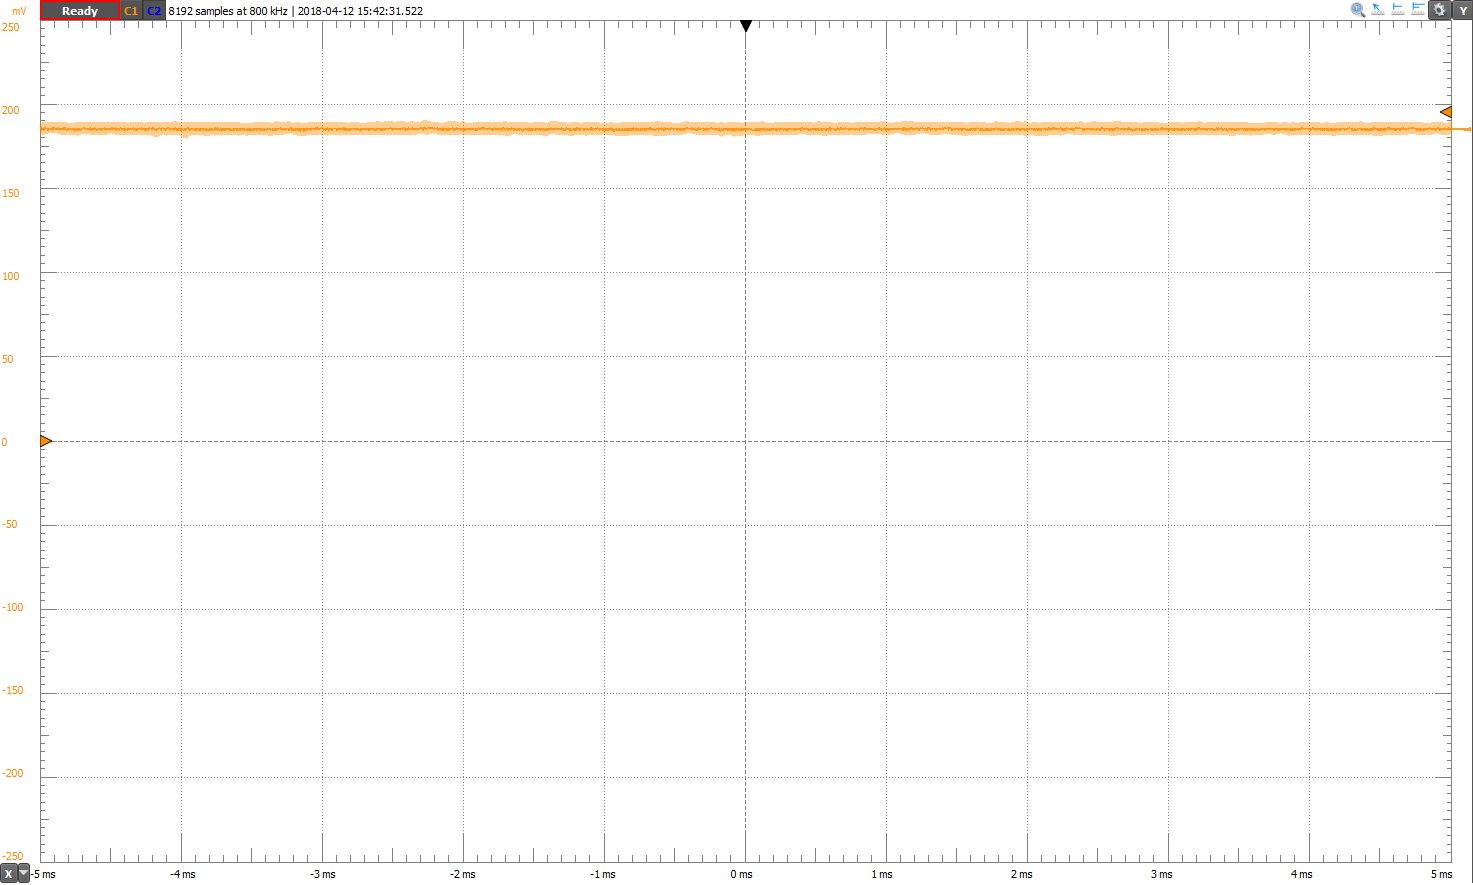
\includegraphics[width=1\linewidth]{implementation/energylab/fig/radioOn_idle.png}
	\caption{Voltage drop at resistor $R=10\Omega$ in series with Receiver (yellow), radio on, doing nothing.}
	\label{fig:radioOn_idle}
\end{figure}

\begin{figure}[H]
	\centering
	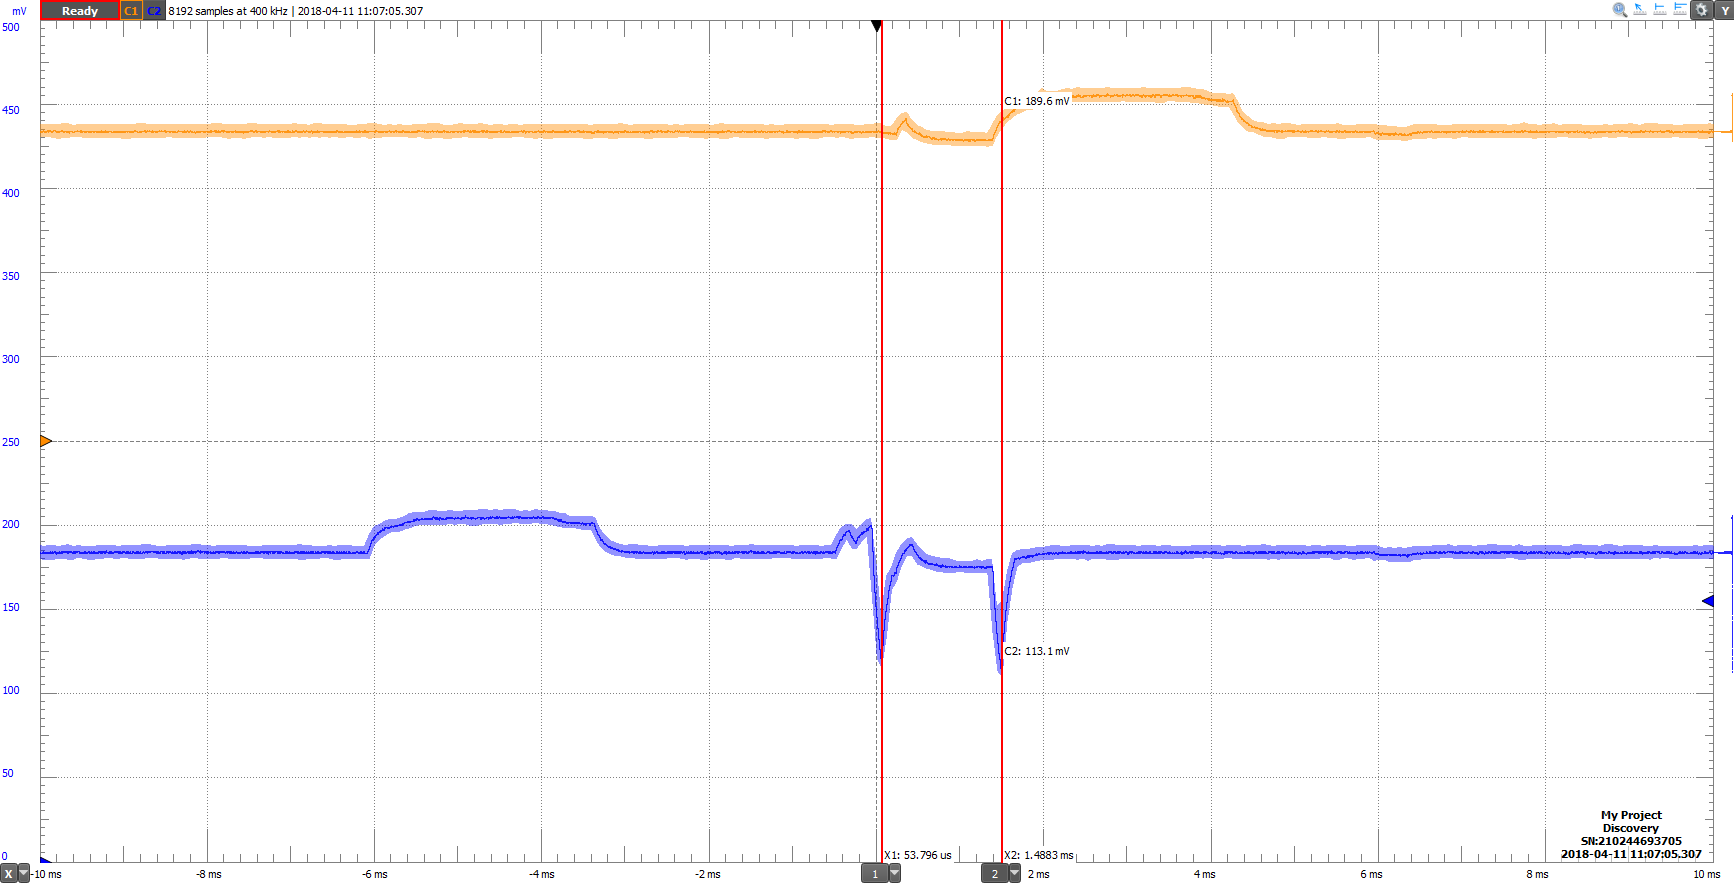
\includegraphics[width=1\linewidth]{implementation/energylab/fig/radioOn_sendHighSignal.png}
	\caption{Voltage drop at resistor $R=10\Omega$ in series with Sender (blue) and Receiver (yellow), radio on, sending at $0.0dBm$.}
	\label{fig:radioOn_sendHighSignal}
\end{figure}

\begin{figure}[H]
	\centering
	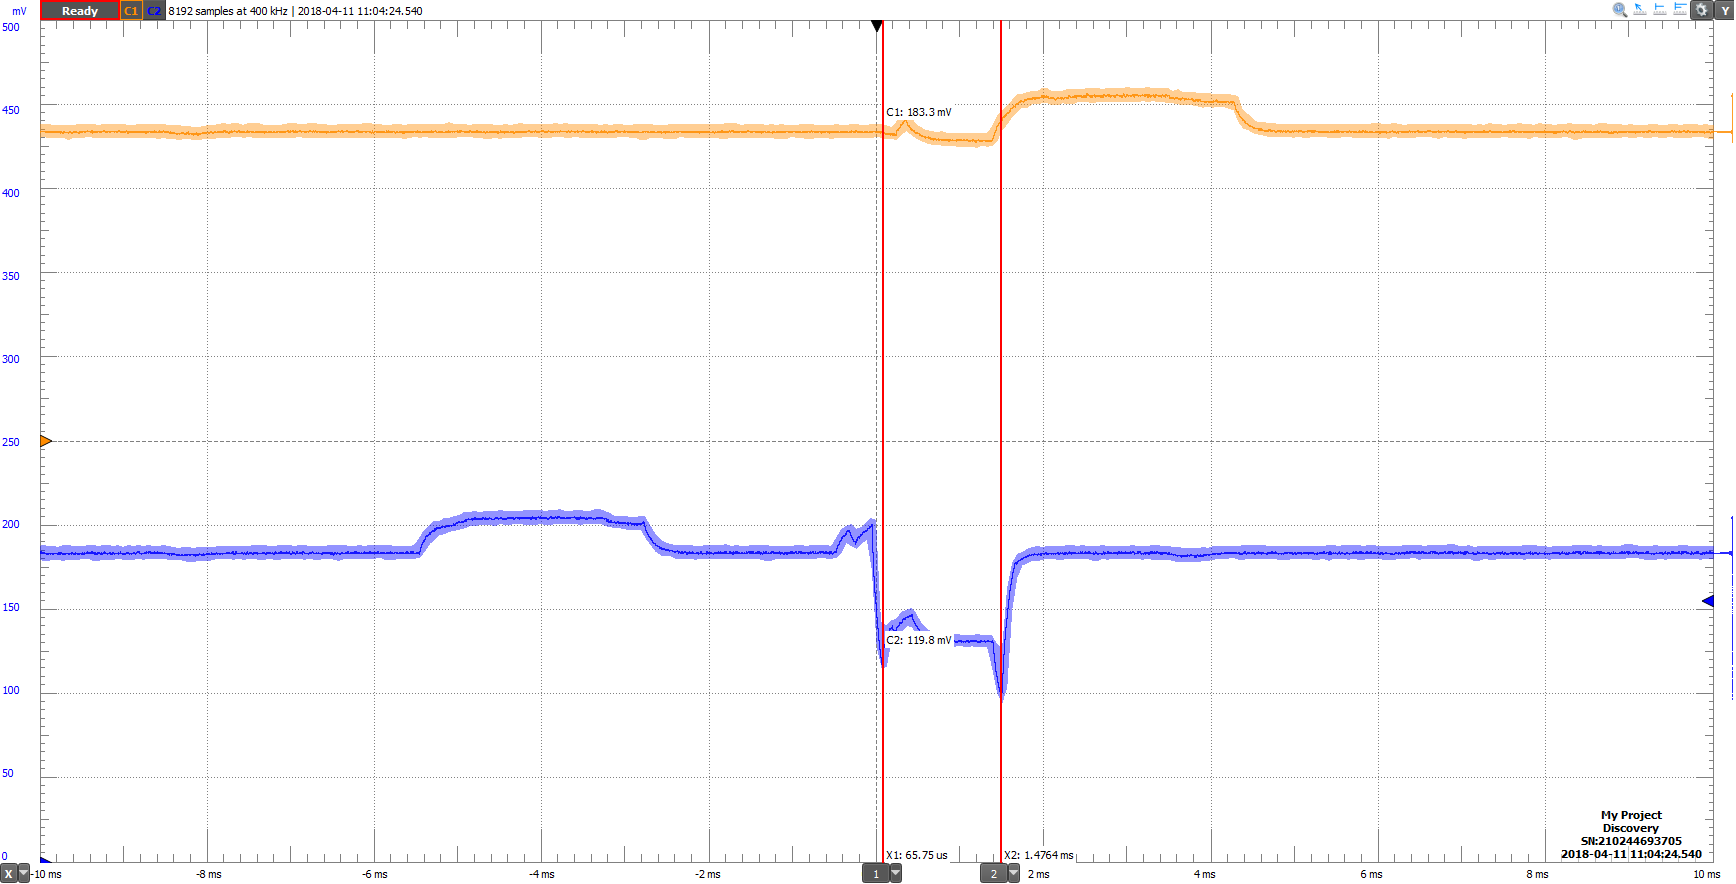
\includegraphics[width=1\linewidth]{implementation/energylab/fig/radioOn_sendMidSignal.png}
	\caption{Voltage drop at resistor $R=10\Omega$ in series with Sender (blue) and Receiver (yellow), radio on, sending at $-12.5dBm$.}
	\label{fig:radioOn_sendMidSignal}
\end{figure}

\begin{figure}[H]
	\centering
	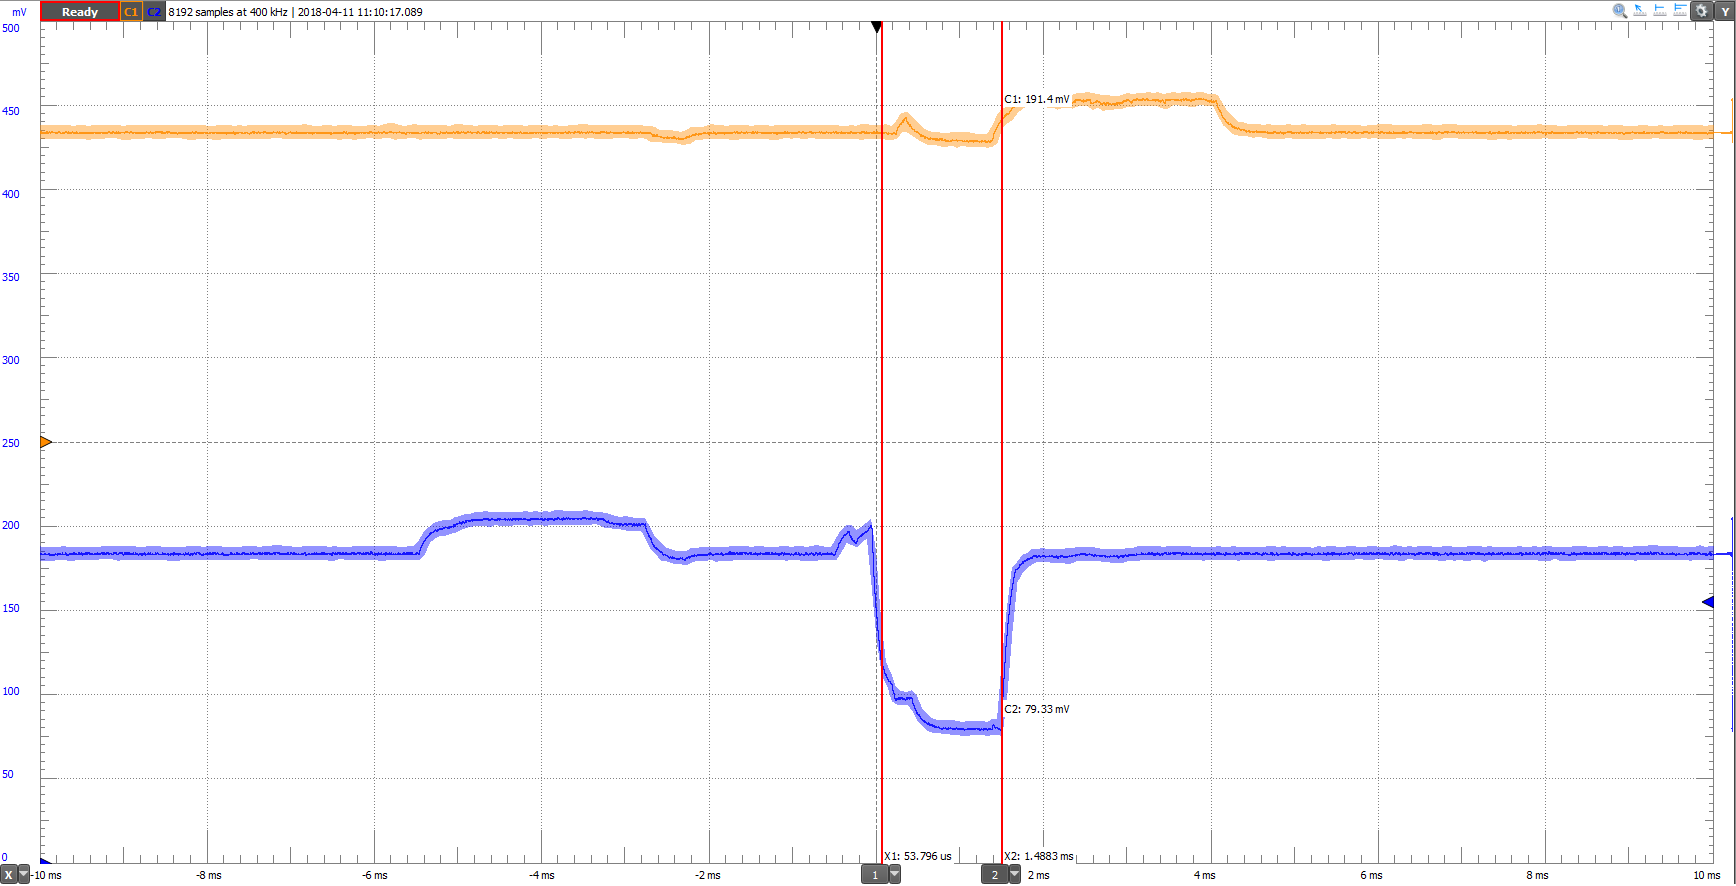
\includegraphics[width=1\linewidth]{implementation/energylab/fig/radioOn_sendLowSignal.png}
	\caption{Voltage drop at resistor $R=10\Omega$ in series with Sender (blue) and Receiver (yellow), radio on, sending at $-25.0dBm$.}
	\label{fig:radioOn_sendLowSignal}
\end{figure}

\begin{table}[H]
	\centering
	\begin{tabularx}{\linewidth}{|X|X|X|}
		\hline
		Radio				& Voltage [mV] at $R=10\Omega$	& Converted Current [mA]	\\ \hline
		OFF					& $3.32$						& $0.33$					\\ \hline
		Listening			& $182.24$						& $18.22$					\\ \hline
		Sending $0.0dBm$	& $172.31$						& $17.23$					\\ \hline
		Sending $-12.5dBm$	& $123.30$						& $12.33$					\\ \hline
		Sending $-25.0dBm$	& $87.20$						& $8.72$					\\ \hline
	\end{tabularx}
	\caption{Mean current drawn from the telosb calculated with voltage drop at resistor $R$.}
	\label{tab:signalStrengthEnergyConsumption}
\end{table}

\noindent Seen in table \ref{tab:signalStrengthEnergyConsumption}, there is a big difference in how much current is drawn at different signal strengths. However at further inspection of the telosb units, it is concluded that turning the radio on, will make a unit automatically start listening for wireless signals. This results in the units always drawing a lot of current whenever the radio is turned on.

\begin{figure}[H]
	\centering
	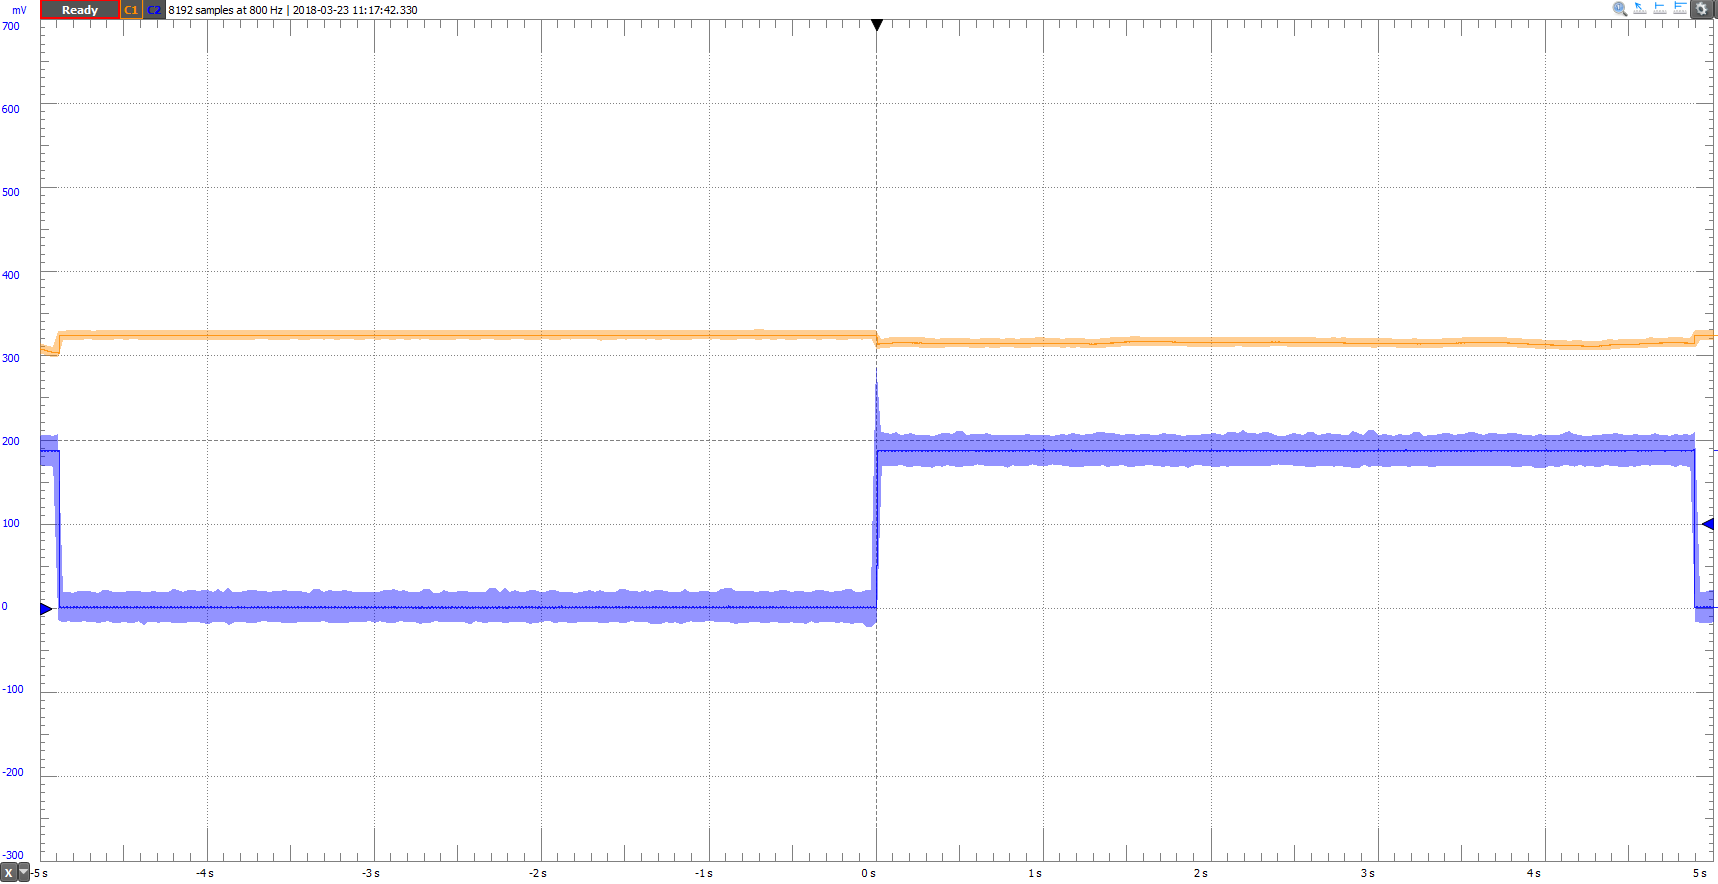
\includegraphics[width=\linewidth]{implementation/energylab/fig/radioSwitching.png}
	\caption{Voltage drop at resistor $R=10\Omega$ in series with telosb unit (blue) and battery (yellow), radio switching between on and off.}
	\label{fig:radioSwitching}
\end{figure}

\noindent As seen in figure \ref{fig:radioSwitching}, turning on the radio is indeed expensive compared to having it turned off. At first thought one might design a protocol that turns off the radio when not needed and on when needed. This will require a protocol with time/clock synchronization of some sort to be implemented, and will not be implemented in this report. An overshoot can be observed at radio turn on, this means that it will cost an extra amount of energy whenever the radio is turned on. This concept have already been talked about in section \ref{sc:energyCalculations} in which the data came from this section.